%!TEX program = xelatex

% \documentclass{ctexart}
\documentclass{article}
% \usepackage[utf8]{inputenc}
\usepackage{xeCJK}

\title{梯度下降总结}
\author{Yuxin Sun}
\date{Jan. 2021}

\usepackage[super,square]{natbib}
\usepackage{graphicx}
\usepackage{amsmath}
\usepackage{geometry}
\usepackage{setspace}
 \geometry{
 a4paper,
%  total={170mm,257mm},
 left=30mm,
 right=30mm,
 top=30mm,
 bottom=25mm
 }
\linespread{1.6}
\newcommand{\E}[1]{\mathrm{E}\left[#1\right]}
\newcommand{\bra}[1]{\left\langle #1\right\rvert}
\newcommand{\ket}[1]{\left\lvert #1\right\rangle}
\begin{document}
\maketitle

\section*{一、梯度下降算法分类}

梯度下降算法根据其对数据的使用方式主要分为三大类: 批量梯度下降法(Batch Gradient Descent), 随机梯度下降法(Stochastic Gradient Descent), 以及小批量梯度下降法(Mini-batch Gradient Descent).
\subsection*{批量梯度下降法}
\begin{equation}
    g_j = \frac{1}{n}\sum_{\sigma=1}^n \nabla f^\sigma(w_j)
\end{equation}
每次求出较为精确的总梯度, 然后计算下一步. 这种方法得到的梯度虽然准确, 但是在将所有样本平均的过程中抹除了每个样本独有的信息, 对数据信息的利用率较低, 因而总计算量较大.

\subsection*{随机梯度下降法}
\begin{equation}
    g_j = \nabla f^{\sigma_j}(w_j)
\end{equation}
每次挑出损失函数特定的部分进行计算, 计算得到的梯度不够准确, 但是大大减少了计算量. 其中$\sigma_j$为随机变量.

\subsection*{小批量梯度下降法}
\begin{equation}
    g_j = \frac{1}{\lvert S\rvert}\sum_{\sigma\in\mathrm{S}} \nabla f^\sigma(w_j)
\end{equation}
可以看做介于以上两种算法之间的方法.

根据算法的原理, 又有各种各样的算法类, 如下图在SDCA下还有其变体MISO方法, 其中有我曾经调研过的Stochastic MISO方法(后来发现不适用于我们的张量网络优化算法).
\begin{figure}[h!]
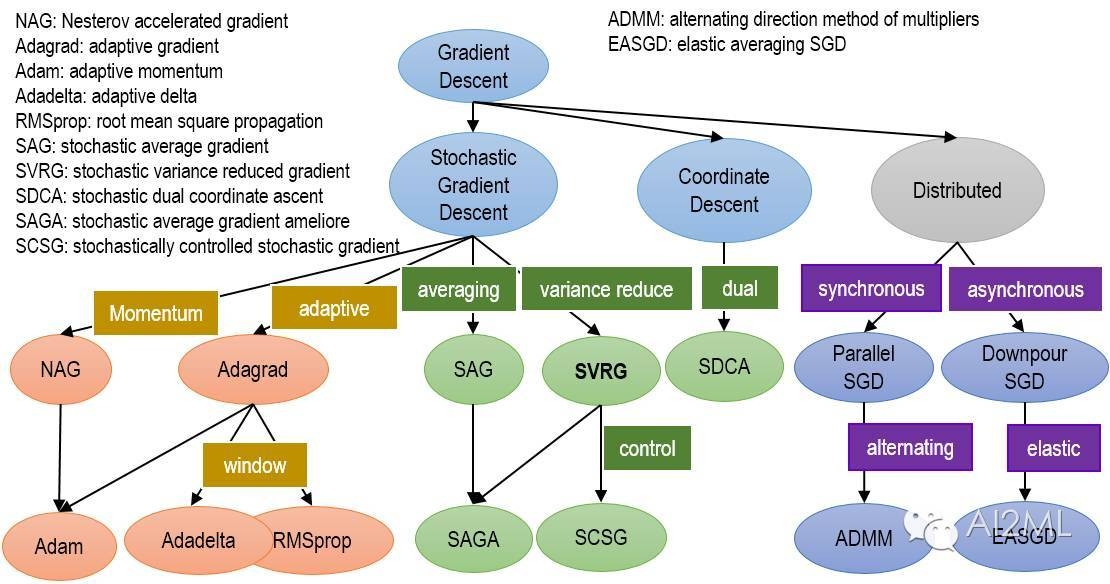
\includegraphics[width=\textwidth]{image/algoFamily.jpeg}
\caption{各种梯度下降算法}
\end{figure}


SVRG算法指出, SGD算法精确度正比于其梯度方差与步长. 在$w$接近极值点时, SGD梯度的方差仍有一个不为零的上界. 
因此想要获得收敛的结果, 算法必须不断缩小步长. 我们尝试一类方差缩减算法, 在计算过程中可以使梯度的方差上界趋于零, 这种算法不用减小步长, 相比于其他算法有更快的收敛速度.
为何选择研究SVRG? 主要出于内存占用方面的考虑. 在详细测试svrg之前, 我们先简单介绍一系列有关算法.

\section*{二、部分算法介绍}

我们主要关注上图中的方差缩减算法.
\subsection*{SAG方法}
\begin{figure}[h!]
    \centering
    \includegraphics[width=\textwidth]{image/algo_SAG.png}
    \caption{SAG}
    \label{fig:SAG}
\end{figure}
待下降函数:
\begin{equation}
    F(w)=\frac{1}{n}\sum_{\sigma=1}^n f^\sigma(w)
\end{equation}

在算法开始时, 我们计算每个$\nabla f^\sigma(w_0)$的值并保存, 记为$\nabla f^{\sigma}$, 之后进入循环, 每次随机选取一个$\sigma_k$, 将$\nabla f^{\sigma_k}$更新为$\nabla f^{\sigma_k}(w_k)$. 之后计算梯度:
\begin{equation}
    g_j = \nabla R_n(w_k)=\frac1n\sum_{\sigma=1}^n \nabla f^\sigma
\end{equation}
这$n$个梯度的平均值中包含了$n-1$个旧梯度与一个刚刚更新过的新梯度的信息.

\subsection*{SAGA方法}

\begin{figure}[h]
    \centering
    \includegraphics[width=\textwidth]{image/SAGA.png}
    \caption{SAGA}
    \label{fig:SAGA}
\end{figure}
这种方法可以看做是修正后的SAG方法, 其每一步在计算出下一个状态后, 并不直接采用, 而是利用 $\text{prox}^h_\gamma(x)$ 对其进行修正. SAG中对梯度的估计不是无偏的, 而SAGA是无偏的. 与SAG相同的是, 我们需要保存$n$份梯度以便替换.

\subsection*{SVRG方法}
\begin{figure}[h]
    \centering
    \includegraphics[width=\textwidth]{image/SVRG.png}
    \caption{SVRG}
    \label{fig:SVRG}
\end{figure}
待下降函数:
\begin{equation}
    F(w)=\frac{1}{n}\sum_{\sigma=1}^n f^\sigma(w)
\end{equation}
\\
在外层循环$j$中, 计算当前状态$w_j$下精确的全梯度:
\begin{equation}
    \nabla R_n(w_j)=\frac1n\sum_{\sigma=1}^n \nabla f^\sigma(w_j)
\end{equation}
\\
在每个$j$中均建立内层循环$k$, 计算 $\nabla f^{\sigma_k}(\tilde{w}_k)$与$\nabla f^{\sigma_j}(\tilde{w}_k)$:
\begin{equation}
    \tilde{g}_k = \nabla R_n(w_j)
        -\nabla f^{\sigma_k}(w_j)
        +\nabla f^{\sigma_k}(\tilde{w}_k)
\end{equation}
\begin{equation}
    \tilde{w}_{k+1}=\tilde{w}_{k}-\alpha \tilde{g}_k    
\end{equation}
\\
和SGD比较: 
\begin{equation}
    g_j = \nabla f^\sigma_j(\tilde{w}_j)
\end{equation}
\begin{align*}
    \E{ \tilde{g}_j} &= \E{\nabla R_n(w_k)
        - \nabla f^{\sigma_j}(w_k)}
        + \E{\nabla f^{\sigma_j}(\tilde{w}_j)}\\
        &= 0 + \E{g_j}\\
        &= \nabla R_n(\tilde{w}_j)
\end{align*}
即每次所得梯度的数学期望与全梯度$\nabla F(w)$方向一致.

\subsection*{SCSG}
SCSG方法(Stochastically Controlled Stochastic Gradient)是SVRG的改进版. 它与SVRG最主要的区别在于其$f^\sigma(w_k)$实际是由SVRG中指定数量的$f^\sigma(w_k)$相加得到的, 
这种处理最终导致其算法复杂度与数据集大小无关, 使其成为一种Online算法, 可以处理数据流.
(需图). 我们做的测试使用一定长度的马尔科夫链代替精确梯度, 可以认为是上文所描述的SCSG方法.

\subsection*{Adam}
另一类算法中的Adam算法, 可认为是一种动量算法.
\begin{figure}[h!]
    \centering
    \includegraphics[width=\textwidth]{image/Adam_algo.png}
    \caption{Adam 算法}
    \label{fig:Adam}
\end{figure}
Adam 算法结合了动量算法与 RMSProp 算法, 通过$m_t$ 对历史梯度进行平均, 防止单次梯度抖动过大, 通过 $v_t$ 对梯度的历史方差进行平均, 自适应调整当前步长大小(注: 这里的$g_t^2$是按元素相乘, 而非内积. 上图中的运算均为按元素运算). 

Adam 算法下降速度一般快于SGD, 但在极值附近的收敛情况可能较差\cite{reddiConvergenceAdam2019}, 因此有论文指出若在梯度下降过程中, 在满足某些条件后将Adam切换为SGD算法, 优于只使用Adam的结果\cite{keskarImprovingGeneralizationPerformance2017}.

另外对于图1中的 AdaDelta, AdaGrad, RMSProp以及上述Adam算法, 文章\citet{reddiConvergenceAdam2019}第3页给出了一个通用公式概括这一类自适应算法的形式.

\subsection*{SVRG与马尔科夫链}
\[F(w)=\frac{1}{n}\sum_{\sigma=1}^n f^\sigma(w)\]
\[\nabla R_n(w)=\frac1n\sum_{\sigma=1}^n \nabla f^\sigma(w)\]
\noindent
我们需要计算
\[
    E = \frac{1}{Z}\sum_S W\!(S)^2 E(S)
\]
以及梯度
\begin{align*}
    \frac{\partial E}{\partial A^{s_m}_{lr}} &= \frac{\partial}{\partial A}\left(\frac{1}{Z}\sum_S W\!(S)^2 E(S)\right)\\
            &= \frac{1}{Z} \frac{\partial}{\partial A} \left(\sum_S W\!(S)^2 E(S)\right) + \frac{\partial}{\partial A}\!\left(\frac{1}{Z}\right)\sum_S W\!(S)^2 E(S)\\
            &= \frac{1}{Z} \sum_S 2W\!(S)\frac{\partial W\!(S)}{\partial A} E(S) - \frac{1}{Z^2}\frac{\partial Z}{\partial A} \sum_S W\!(S)^2 E(S)\\
            &= 2\,\frac{1}{Z}\!\sum_S W\!(S)^2\left(\frac{1}{W\!(S)}\frac{\partial W\!(S)}{\partial A}\right) E(S) \\
                &\quad - \frac{1}{Z^2}\frac{\partial}{\partial A}\left(\sum_S W\!(S)^2\right) \sum_S W\!(S)^2 E(S)\\
            &= 2\,\frac{1}{Z}\!\sum_S W\!(S)^2\Delta(S) E(S) \\
            &\quad - 2\,\frac{1}{Z^2}\! \sum_S W\!(S)^2\Delta(S) \sum_S W\!(S)^2 E(S)\\
            &= 2\langle{\Delta}^{s_m}_{lr}(S)E(S)\rangle -  2\langle{\Delta}^{s_m}_{lr}(S)\rangle\langle E(S)\rangle
\end{align*}
其中
\[
    E(S) = \sum_{S'}\frac{W\!(S')}{W\!(S)}\bra{S'}\mathbf{H}\ket{S}
\]
将这里的$Z=W(S)^2$ 看做配分函数,
利用马尔科夫链构造$W(S)^2$为权重的抽样, 对应每个自旋构型下样本$E(S)=E_s$, 公式可以简化为
\[
    E = \frac{1}{n}\sum_s E_s
\]
\[
    \frac{\partial E}{\partial A} = 2\left(\frac{1}{n}\sum_s \Delta_s E_s -\frac{1}{n}\sum_s \Delta_s\cdot\frac{1}{n}\sum_s E_s\right)
\]
上述梯度在每个样本$s$出现的频率严格等于概率时, 严格等于张量网络的梯度. 我们将上式记为$f(w_k; \xi_k)$, 即该梯度是关于张量网络状态$w_k$与马尔科夫链$\xi_k$的函数, 其随机性来自马尔科夫链, 期望值约等于梯度.
仿照公式(8), 我们构造梯度
\begin{equation}
    g(w_j) = \nabla R(w_\text{old}) - f(w_\text{old}; \xi_\text{old}) + f(w_j; \xi_j)
\end{equation}
这里的$f(w; \xi)$对应原始SVRG中的随机梯度$f^{\sigma}(w)$. 为了节省计算量, 我们将对式中最后一项使用reweighting方法, 利用计算$\xi_\text{old}$时生成的马尔科夫链, 得到当前$\xi_j$下的物理量.


\section*{三、测试数据}
下面计算海森堡模型$\hat{H}=J\sum_i \vec{\sigma}_i\cdot\vec{\sigma}_{i+1}$的基态. 

\subsection*{1. 令$J = -1$}
\subsubsection*{OBC}
基态时相邻自旋平行, 呈铁磁相. 首先测试一个小系统中算法是否正常工作:
\begin{figure}[!ht]
    %\centering
    \includegraphics[width=0.48\textwidth]{image/sgd.pdf}
    \includegraphics[width=0.48\textwidth]{image/svrg_rand.pdf}
    \caption{SGD and SVRG with stochastic gradient $\nabla R$}
    \label{fig:SGD_SVRG}
\end{figure}

\noindent
增加MPS长度, SGD:
\begin{figure}[h!]
    \centering
    \includegraphics[width=0.48\textwidth]{image/sgd3.pdf}
    \includegraphics[width=0.48\textwidth]{image/sgd4.pdf}
    \caption{SGD, 其中左图接近最优步长, 右图步长与下文SVRG相等}
    \label{fig:SGD3}
\end{figure}

随机梯度下的SVRG:
\begin{figure}[h!]
    \centering
    \includegraphics[width=0.9\textwidth]{image/svrg_rand3.pdf}
    \caption{SVRG with stochastic gradient $\nabla R$}
    \label{fig:SVRG_rand02}
\end{figure}

\clearpage

\noindent
另外测试了一下 SVRG 原论文\cite{johnsonAcceleratingStochasticGradient}中要求的使用严格梯度的方法(此方法不适用于张量网络, 因为用非随机算法直接计算张量网络非近似的梯度复杂度过高).
\begin{figure}[!ht]
    \centering
    \includegraphics[width=\textwidth]{image/svrg_exact.pdf}
    \caption{SVRG with exact gradient $\nabla R$}
    \label{fig:SVRG_rand}
\end{figure}
经过测试, 这个算法比使用随机梯度的SVRG更加稳定, 下降速度更快, 对步长要求小, 但由于前述原因, 在之后的实验中不再考虑.

对更大一点的系统进行测试时, 我们希望从一个适当的初态开始, 因此这里对一个随机初态进行大致的梯度下降, 得到一个适当的初态用于之后的测试.
\begin{figure}[!ht]
	\centering
	\includegraphics[width=0.9\textwidth]{./image/preSGD_OBC_ferro.pdf}
	\caption{Get a low energy state by SGD preprocessing.}
\end{figure}

\clearpage\noindent
测试结果(由于是之后补充的测试, 因此测试时加上了Adam算法, 可以看出Adam的优势):
\begin{figure}[!ht]
	\centering
	\includegraphics[width=\textwidth]{./image/comparison_ferro_opc.pdf}
	\caption{Comparison of three algorithms. y: $\log\lvert E-E_0\rvert$, x: steps }
	\label{fig:comp1}
\end{figure}

图11中, 随着步长增大, 算法效率先提高后下降, 因此可以猜测最优步长在一、三两行对应步长之间. 对比第二行的两张图, 可以发现增大采样数量可以较好的保证算法的线性收敛性. 另外第三行中, SVRG算法出现抖动, 此时步长过大, 算法变得不稳定.

\clearpage
\subsubsection*{PBC}

将MPS改为周期边界条件, 测试算法在不同结构下的性能. 在PBC中我们无法利用MPC的正则形式快速算出能量的准确值, 计算时间相比于OBC有所增加. 为了节省计算量, 能量的数值根据梯度下降时的采样数据得出. 由于并非准确值, 这里的绘图方式由 Plot 改为了 Scatter.

\begin{figure}[!h]
	\centering
	\includegraphics[width=\textwidth]{image/sgd_adam_43.pdf}
	\caption{SGD 与 Adam 比较, y轴为$\log\lvert E-E_0 \rvert$.}
	\label{fig:SGD_Adam_PBC}
\end{figure}
Adam算法明显优于SGD.

\clearpage
\subsection*{2. 令$J = 1$}
由于查不到OBC时的基态能量与系统大小$N$ 的关系, 没法画出能量对数图比较收敛速度, 因此跳过OBC的测试, 直接在PBC条件下测试. 此时的基态趋向于相邻自旋反平行. 

\begin{figure}[!h]
	\centering
\includegraphics[width=\textwidth]{image/sgd_adam_antiferro_pbc.pdf}
	\caption{SGD 与 Adam 比较, y轴为$\log\lvert E-E_0 \rvert$.}
	\label{fig:SGD_Adam_PBC}
\end{figure}
Adam在此条件下略快于SGD. 但性能没有显著优越性.

另外董师兄就此条件利用其函数库的实际代码进行了测试, 初步测试结果为, 在相同步长参数下两者没有明显差异. 

对于两者在各自最优参数下的比较暂缺.

\clearpage


% \begin{figure}[h!]
% \centering
% \includegraphics[scale=1.7]{universe}
% \caption{The Universe}
% \label{fig:universe}
% \end{figure}

\bibliographystyle{unsrt}
\bibliography{references}
\end{document}
